\documentclass[pdf,aspectratio=169]{beamer}
\usepackage[]{hyperref,graphicx,siunitx,lmodern,booktabs,tikz,tensor}
\usepackage{pdfpc-commands}
\usepackage{pgfplots, pgfplotstable}

\usepackage[mode=buildnew]{standalone}
\mode<presentation>{\usetheme{Astro}}

\graphicspath{ {../Images/} }

\sisetup{per-mode=symbol, group-separator={,}}
\usetikzlibrary{calc,intersections, decorations.pathmorphing,shadings,positioning}
%\tikzstyle{proton}=[circle, minimum size = 7mm, ball color=red, black,transform shape]
%\tikzstyle{neutron}=[circle, minimum size=7mm, ball color=gray, black, transform shape]
%\tikzstyle{gammaray}=[ultra thick, -latex, decorate, decoration={snake, post length=3mm}]


%preamble
\title{Wrinkles in Time (and Space!)}
\date{December 3, 2018}
\author{Jed Rembold}

\begin{document}
\renewcommand*{\theenumi}{\Alph{enumi}}

\begin{frame}{Announcements}
  \begin{itemize}
	\item Webwork due on Wednesday
	\item Last week of lab for Group B!
	\item Final one week from Wednesday
	  \begin{itemize}
		\item 8am in this room
		\item Technically have 3 hours, but I write for 1.5x or 2x normal test length
		\item Last study materials will be posted tomorrow
		\item Cumulative, but about 1/3 will be focused on most recent content (galaxies and cosmology)
	  \end{itemize}
	\item Polling: \url{rembold-class.ddns.net}
  \end{itemize}
\end{frame}

\begin{frame}{Galaxy Spins}
	\begin{columns}
		\column{0.5\textwidth}
		\inlineMovie{../Videos/wind.ogv}{../Videos/wind.png}{width=\textwidth}
		\column{0.5\textwidth}
		\inlineMovie{../Videos/wave.ogv}{../Videos/wave.png}{width=\textwidth}
		
	\end{columns}
\end{frame}

\begin{frame}{Review Question}
  How fast is a galaxy retreating from us if it is located \SI{300}{\mega pc} away? 
  \begin{enumerate}
	\item \SI{4.167}{\kilo\meter\per\second}
	\item \SI{4167}{\kilo\meter\per\second}
	\item \alert<2>{\SI{21600000}{\meter\per\second}}
	\item \SI{21600000}{\kilo\meter\per\second}
  \end{enumerate}
\end{frame}

\begin{frame}{The Hubble Xtreme Deepspace 3D!}
  \begin{center}
	\inlineMovie{../Videos/deepfield_fly.ogv}{../Videos/deepfield_fly.png}{width=.8\textwidth}
  \end{center}
\end{frame}

\begin{frame}{A Trip Down Memory Lane}
  \begin{center}
	\includegraphics[width=.9\textwidth]{ch16_hubble_early_universe.jpg}
  \end{center}
\end{frame}

\begin{frame}{Galaxy Evolution Detour}
  \begin{itemize}
	\item Build up a sort of yearbook of galaxy ages
	  \begin{itemize}
		\item Looking at more distance objects means we are looking at younger objects
	  \end{itemize}
	\item Do we see a trend between spiral, elliptical and irregular galaxies over time?
	  \begin{itemize}
		\item Not really, they all follow their own path
	  \end{itemize}
	\item So why the different types?
  \end{itemize}
\end{frame}

\begin{frame}{A Product of their Time}
  \begin{itemize}
	\item Two main ideas though to determine galaxy type:
	  \begin{itemize}
		\item \textcolor{Orange}{Initial rotation rate:} Perhaps with a small enough angular momentum, galactic disks never form and they stay elliptical
		\item \textcolor{Orange}{Initial density:} Clouds with a high gas density would have formed stars much faster, and maybe used up all the gas before it had a chance to collapse into a disk
	  \end{itemize}
	\item Observations of a few massively redshift elliptical galaxies:
	  \begin{itemize}
		\item Lack blue and white stars
		\item Even though universe still quite young
		\item Supports fast star formation theory?
	  \end{itemize}
	\item Collisions and gravitational tugs likely played major roles in subsequent shaping
  \end{itemize}
\end{frame}

\begin{frame}{Back to the Universe: A Slowing Expansion?}
  \begin{itemize}
	\item We've been assuming that space expands at a constant rate
	\item But gravity is attractive, and should be slowing that expansion?
	\item Are we overestimating the lifetime of the universe?
  \end{itemize}
\end{frame}

\begin{frame}{Ultimate Questions of the Universe}
  \begin{itemize}
	\item Is it infinite?
	\item Is it curved or flat?
	\item Is it growing or shrinking?
	\item What is the whole deal with this Big Bang thing?
  \end{itemize}
\end{frame}

\begin{frame}{Mass: Forever the Answer}
  \begin{itemize}
	\item The simplest GR models predict that expansion will slow
	  \begin{itemize}
		\item Gravity will slowly win, at a rate dependent on the mass density ($\Omega$) of the universe
	  \end{itemize}
	%\item The mass density also determines the geometry of the universe
  \end{itemize}
  \begin{center}
	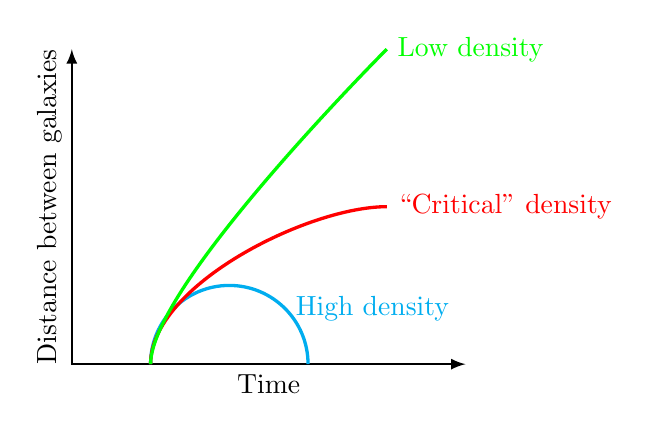
\begin{tikzpicture}
	  \draw[thick, latex-latex] (5,0) -- (0,0) node[midway, below] {Time} -- (0,4) node[midway,sloped,above] {Distance between galaxies};
	  \draw[cyan, very thick] (1,0) arc (180:0:1) node[near end, right] {High density};
	  \draw[red, very thick] (1,0) ..controls +(90:1) and +(180:1).. (4,2) node[right] {``Critical'' density};
	  \draw[green, very thick] (1,0) ..controls +(90:1) and +(180:0).. (4,4) node[right] {Low density};
	\end{tikzpicture}
  \end{center}
\end{frame}

\begin{frame}{Curved Geometry}
  \begin{columns}
	\column{.5\textwidth}
	\begin{itemize}
	  \item The mass density also determines the shape of the universe:
		\begin{itemize}
		  \item \textcolor{Orange}{$\Omega>1$} implies a positive curvature
		  \item \textcolor{Orange}{$\Omega<1$} implies a negative curvature
		  \item \textcolor{Orange}{$\Omega=1$} implies no curvature (flat)
		\end{itemize}
	\end{itemize}
	\column{.5\textwidth}
	\begin{center}
	  \includegraphics[width=\textwidth]{ch18_curvature.png}
	\end{center}
  \end{columns}
\end{frame}

\begin{frame}{Measuring Curvature}
  \begin{itemize}
	\item There are several approaches to measuring $\Omega$:
	  \begin{itemize}
		\item Look at all the mass, and figure out a density directly
		  \begin{itemize}
			\item From visible mass $\Omega\approx 0.02$
			\item Including dark mass $\Omega\approx 0.3$
		  \end{itemize}
		\item Try to measure very precise triangles to look for angles $>$ or $<\SI{180}{\degree}$
		\item Look for changes in the expansion rate: the ``deceleration parameter'' $q_0$
	  \end{itemize}
  \end{itemize}
	\begin{center}
	  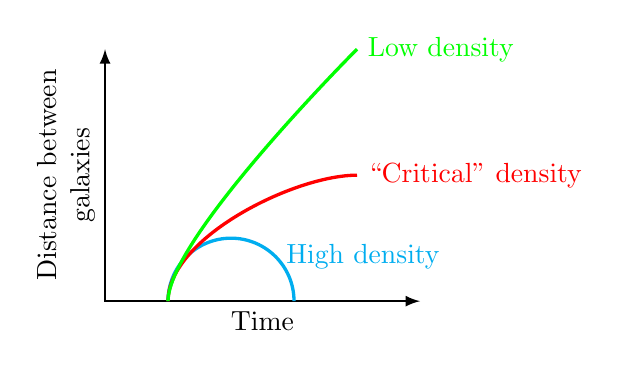
\begin{tikzpicture}[scale=0.8]
		\draw[thick, latex-latex] (5,0) -- (0,0) node[midway, below] {Time} -- (0,4) node[midway,sloped,above,align=center] {Distance between\\galaxies};
		\draw[cyan, very thick] (1,0) arc (180:0:1) node[near end, right] {High density};
		\draw[red, very thick] (1,0) ..controls +(90:1) and +(180:1).. (4,2) node[right] {``Critical'' density};
		\draw[green, very thick] (1,0) ..controls +(90:1) and +(180:0).. (4,4) node[right] {Low density};
	  \end{tikzpicture}
	\end{center}
\end{frame}

\begin{frame}{A Geometrical Conundrum!}
  \begin{itemize}
	\item Based off all our adding up of the masses, including dark matter we have a density of $\Omega \approx 0.3$
	  \begin{itemize}
		\item This would imply an open, negative curvature universe
	  \end{itemize}
	\item Very recent results from Baryon Acoustic Oscillation (BAO) work though has the universe being flat to within 0.4\% probability
	\item Are we missing something? Or is some physical law flawed?
  \end{itemize}
\end{frame}

\begin{frame}{Return of the Hubble}
  \begin{columns}
	\column{.5\textwidth}
	\begin{itemize}
	  \item GR predicts gravity should slow expansion
	  \item Looking at the Hubble Relation out to very large distances then, we don't expect a straight line
	  \item Measuring that deviation from straight has been a long-standing goal of observational cosmology!
	\end{itemize}
	\column{.5\textwidth}
	\begin{center}
	  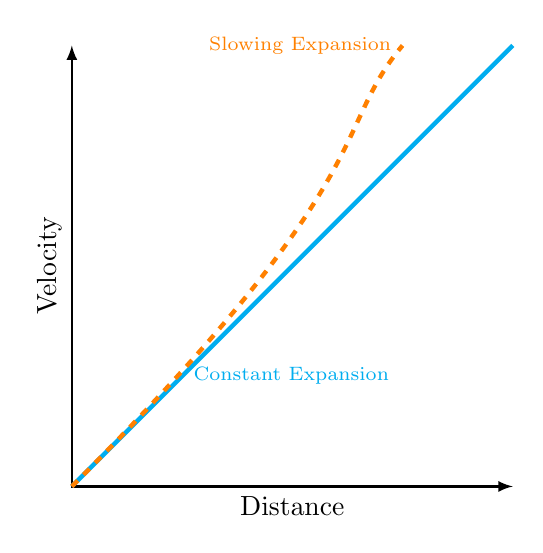
\begin{tikzpicture}[scale=1.4]
		\draw[thick, latex-latex] (4,0) -- (0,0) node[midway,below] {Distance} -- (0,4) node[midway,sloped,above] {Velocity};
		\draw[cyan,ultra thick] (0,0) -- (4,4) node[near start, right, font=\scriptsize] {Constant Expansion};
		\draw[orange, dashed, ultra thick] (0,0) ..controls +(45:4) and +(230:1).. (3,4) node[left, font=\scriptsize] {Slowing Expansion};
	  \end{tikzpicture}
	\end{center}
  \end{columns}
\end{frame}

\begin{frame}{And the results are in!}
  \begin{itemize}
	\item So what did astronomers finally see?
  \end{itemize}
  \begin{center}
	\begin{tikzpicture}
	  \begin{axis}[
		  height=6cm,
		  width=9cm,
		  scaled x ticks=false,
		  xlabel = Distance (Mpc),
		  ylabel = Redshift (z),
		  xticklabel style = {rotate=90, font=\scriptsize},
		  xlabel near ticks,
		]
		\addplot[orange!50!black, fill=orange,only marks] table[x index=1, y index=0] {../Data/HubbleExpand.csv};
		\addplot[very thick, cyan, domain=0:12000, samples=50] {x*52.65/3e5};
	  \end{axis}
	\end{tikzpicture}
  \end{center}
\end{frame}

\begin{frame}{Oh \#@*\$! What?!}
  \begin{itemize}
	\item Recent observations (1998) suggest expansion is \alert{not} slowing
	  \begin{itemize}
		\item The expansion rate is now higher than it was in the past!
		\item $q_0<0$
		\item Universe may actually be \emph{older} than Hubble time?
	  \end{itemize}
	\item \alert{None} of the basic GR models predicted this
	\item Was Einstein's ``cosmological constant'' correct after all?
  \end{itemize}
  \begin{center}
	\begin{tikzpicture}
	  \node[inner sep=0pt, outer sep=0pt] at (0,0) {\includegraphics[width=6cm]{ch18_fieldeqns.jpg}};
	  \node[orange] at (6,0) {$\displaystyle R_{ab}-\frac{1}{2}Rg_{ab} = -8\pi T_{ab} + \color{Blue}\Lambda g_{ab}$};
	\end{tikzpicture}
  \end{center}
\end{frame}

\begin{frame}{So how do we explain this?}
  \begin{center}
	\begin{tikzpicture}
	  \begin{axis}[
		  width=10cm,
		  height=7cm,
		  scaled y ticks=false,
		  xlabel = Distance (Gpc),
		  ylabel = cz (km/s),
		  ylabel near ticks,
		  legend pos = south east,
		  legend style = {fill=none, draw=none, font=\scriptsize},
		  xmin=0, ymin=0,
		]
		\addplot[Foreground, only marks] table[x index=0, y index=1] {../Data/SNData.csv};
		\only<2>{
		\addplot[mark=none, violet!70, very thick] table[x index=0, y index=1] {../Data/FlatDarkEnergy.csv};
		\addplot[mark=none, orange!70, very thick] table[x index=0, y index=1] {../Data/ClosedDarkEnergy.csv};
		\addplot[mark=none, red, very thick] table[x index=0, y index=1] {../Data/ClosedMatterOnly.csv};
		\addplot[mark=none, cyan, very thick] table[x index=0, y index=1] {../Data/deSitterModel.csv};
		\legend{Supernova Data, Flat with Dark Energy, Closed with Dark Energy, Closed Matter Only, de Sitter Model};
	  }
	  \end{axis}
	\end{tikzpicture}
  \end{center}
\end{frame}

\begin{frame}{Dark Energy}
  \begin{itemize}
	\item Of the many models so far put forth, adding dark energy to GR for a flat universe gives the greatest agreement with observations
	\item Dark energy is excess energy that is pushing the universe outward
	  \begin{itemize}
		\item Similar to how gas pressure pushes stars outward
	  \end{itemize}
	\item No idea yet of the source of this energy
	  \begin{itemize}
		\item Energies are tied to forces
		\item No known forces would result in this invisible and excess energy!
	  \end{itemize}
  \end{itemize}
\end{frame}

\begin{frame}{The Galactic Timeline}
  \begin{center}
	\begin{tikzpicture}
	  \begin{axis}[
		  width=10cm,
		  height=7cm,
		  xlabel= Billions of Years,
		  ylabel= Relative Size of Universe,
		  ymin=0.1, ymax=4,
		  xmax=30,
		]
		\addplot[mark=none, red, ultra thick] table[x index=0, y index=1] {../Data/3and7.csv};
		\addplot[mark=none, cyan, ultra thick] table[x index=0, y index=1] {../Data/3and0.csv};
		\addplot[mark=none, green, ultra thick] table[x index=0, y index=1] {../Data/1and0.csv};
		\addplot[mark=none, orange, ultra thick,smooth] table[x index=0, y index=1] {../Data/5and0.csv};
		\node (1) at (axis cs: -8,3.5) {$\Omega_m \qquad \Omega_v$};
		\node[below =0.5mm of 1,red] (2) {0.3\qquad0.7};
		\node[below =0.5mm of 2,cyan] (3) {0.3\qquad0.0};
		\node[below =0.5mm of 3,green] (4) {1.0\qquad0.0};
		\node[below =0.5mm of 4,orange] (4) {5.0\qquad0.0};
	  \end{axis}
	\end{tikzpicture}
  \end{center}
\end{frame}

\begin{frame}{Flat and Expanding}
  \begin{itemize}
	\item Note that the sum of the two density factors now gives a value of 1
	  \begin{itemize}
		\item Supporting the findings that the universe seems to be flat!
	  \end{itemize}
	\item Dark energy provides the extra 70\% of the mass/energy of the universe
	\item Results in an age of the universe very similar to the 14 billion years estimated from a constant expansion rate
	\item So, as far as we know, at the moment we think that our universe is:
	  \begin{itemize}
		\item Flat
		\item Expanding increasingly quickly
		\item About 14 billion years old
		\item Infinite or Finite is not well determined yet
	  \end{itemize}
  \end{itemize}
\end{frame}

%\begin{frame}{Understanding Check}
  %In the absence of dark energy, suppose that we had found strong evidence that our universe had positive curvature ($\Omega_m > 1$). How would the age of such a universe compare to our own?
  %\begin{enumerate}
	%\item It would be much older
	%\item It would be about the same age
	%\item \alert<2>{It would be much younger}
	%\item Time would be flowing backwards, so it would be hard to tell
  %\end{enumerate}
%\end{frame}

%\begin{frame}{Taking it Back}
  %\begin{columns}
	%\column{.5\textwidth}
	%\begin{itemize}
	  %\item Long ago the universe was denser
	  %\item And hotter
	  %\item Can we look back far enough to ``see'' this ``era''?
	%\end{itemize}
	%\column{.5\textwidth}
	%\begin{center}
	  %\includegraphics[width=\textwidth]{ch18_expanding.png}
	%\end{center}
  %\end{columns}
%\end{frame}

%\begin{frame}{Physics In Reverse}
  %\begin{itemize}
	%\item Moving backwards, and using what we know about stars, nuclear physics, and everything else, the history of the universe looks something like below:
  %\end{itemize}
  %\begin{center}
	  %\begin{tikzpicture}
		  %\node[inner sep=0pt, outer sep=0pt](pic1) at (0,0) {\includegraphics[width=.495\textwidth]{ch18_universehistory1.jpg}};
		  %\node[inner sep=0pt, outer sep=0pt,anchor=west] at (pic1.east) {\includegraphics[width=.495\textwidth]{ch18_universehistory2.jpg}};
	  %\end{tikzpicture}
	%%\includegraphics[width=.495\textwidth]{ch18_universehistory1.jpg}
	%%\includegraphics[width=.495\textwidth]{ch18_universehistory2.jpg}
  %\end{center}
%\end{frame}

%\begin{frame}{How far back COULD we see?}
  %\begin{itemize}
	%\item Assuming perfect and huge telescopes, how far back could we see?
	%\item Early universe very very hot
	  %\begin{itemize}
		%\item Hot enough for fusion
		%\item Hot enough that particles charged
		%\item Fusion releases radiation, that interacts with particles
		%\item Light gets scattered $\Rightarrow$ opaque
	  %\end{itemize}
	%\item Once it cooled enough for non-ionized atoms to form, radiation no longer interacts
	  %\begin{itemize}
		%\item Can travel long distances
		%\item Transparent
	  %\end{itemize}
	%\item Called ``Recombination''
  %\end{itemize}
%\end{frame}

%\begin{frame}{Recombination}
  %\begin{center}
	%\includegraphics[width=.6\textwidth]{ch18_recombination.png}
  %\end{center}
%\end{frame}



\end{document}
